%!TEX root = ../MasterThesis.tex

\section{An \gls{ER} model for \gls{E-commerce} transactions}
\label{sec:data_model_transactions}

Based on the analysis of the information each stakeholder holds and transmits to others in Section~\ref{sec:stakeholder_analysis}, the following \gls{ER} model can be conducted for \gls{E-commerce} transactions (see Figure~\ref{fig:images_data_model}). This figure shows not only the relevant information from the local contexts of each stakeholder, but also how they can be combined within a shared information space. \\

\begin{figure}[!ht]
  \centering
  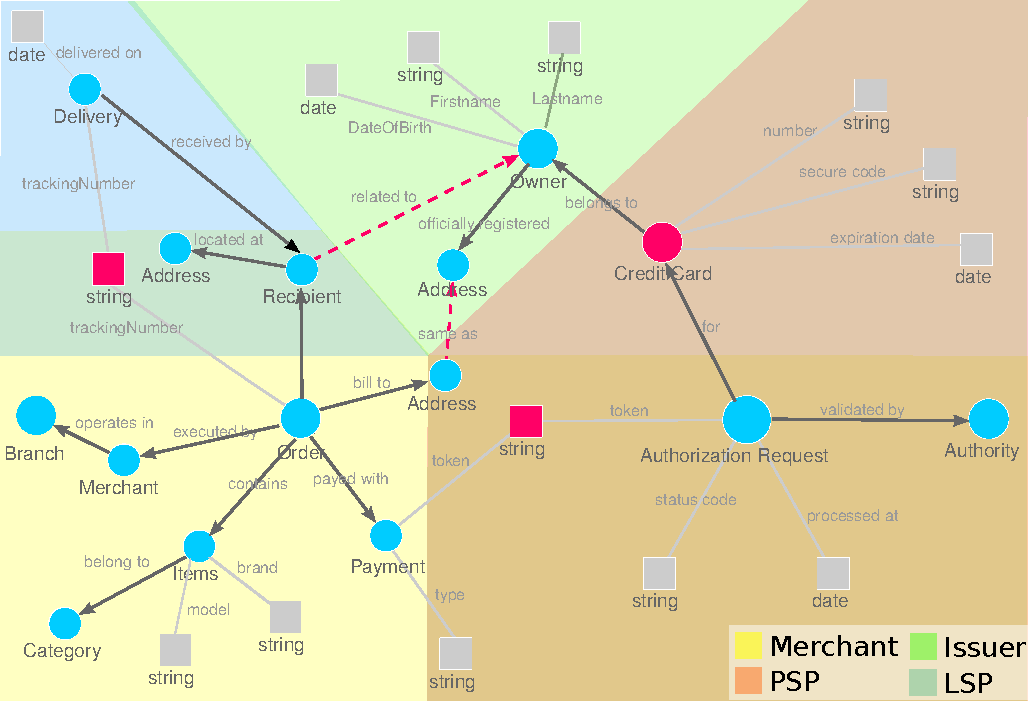
\includegraphics[width=0.9\columnwidth]{images/ontology_scenario_1.pdf}
  \caption[Entities and relations in the \gls{E-commerce} scenario]{Entities and relations in the \gls{E-commerce} scenario}
\label{fig:images_data_model}
\end{figure}

As the figure also shows there are \emph{shared information tokens} that will be exchanged between various stakeholders. Those can be used in the collaborative system as a reference for joining the distributed pieces of information into a combined view of an \gls{E-commerce} transaction. There are actually three important tokens: \@

\begin{enumerate}
  \item \textbf{payment token}: shared between merchants and \gls{PSP}s,
  \item \textbf{tracking number}: shared between merchants and \gls{LSP}s,
  \item \textbf{credit card}: shared between issuers and \gls{PSP}s
\end{enumerate}

In addition to these tokens Figure~\ref{fig:images_data_model} also shows the important validation criteria. These are two important connections that have an influence on the decision whether an \gls{E-commerce} transaction is evaluated as fraudulent or not. The two main criteria are: \@

\begin{enumerate}
  \item \textbf{billing address-to-owner address}: the billing address of the order has to match the registered address of the credit card owner
  \item \textbf{recipient-to-owner}: the recipient of the delivery has to be related to the owner of the credit card
\end{enumerate}

Whereas the first criteria can be examined during the payment authorization process of an \gls{E-commerce} transaction based on the information transmitted between merchants and \gls{PSP}s or issuers, the second one is more difficult to validate (or can not be verified at all). The only check the \gls{LSP}s are able to do, before they are handing over the packaged items to the recipients, is to verify that they are the ones mentioned in the shipping address information of the order. If a recipient is somehow related to the owner of the credit card used for paying an order, or just a deceiver misusing a credit card can not be confirmed by the \gls{LSP}. \\

Also merchants, \gls{PSP}s and issuers have no possibility to check for this criteria. Whereas the merchants are able to validate whether a consumer has send items to a shipping address before, they can not restrict consumers to choose only validated recipient addresses for their orders. Doing so would have negative impacts on the business success of the online merchant. The \gls{PSP}s and issuers can not analyse this situation either, because both participants will not receive any information about the delivery address of an order with the payment authorization request from a merchant. \\

But just sharing the fact whether the shipping and billing address of an order is different or not between the relevant stakeholders is not enough. Although this information is necessary, it is not sufficient to make a decision about suspicious transactions. Other necessary information are whether the consumer has send orders to this shipping address before, and information about the content of the current order. Nevertheless, as mentioned in Section~\ref{sec:scope_thesis} looking at the transactions of just one of the online merchants is not enough either to solve the \gls{E-commerce} fraud scenario, that this Master Thesis looks at. More sophisticated analysing capabilities are required for the collaborative system to be helpful for the \gls{E-commerce} fraud investigation.

% section system_overview (end)
